\documentclass[11pt]{article}
\usepackage[margin=1in]{geometry}
\usepackage{xcolor}
\usepackage{enumitem}
\usepackage{fontawesome5}
\usepackage{titlesec}
\usepackage{multicol}
\usepackage{graphicx}
\usepackage{tikz}
\usepackage{fancyhdr}
\usepackage{lastpage}
\usepackage{tabularx}
\usepackage{booktabs}

% Color definitions
\definecolor{serpentgreen}{RGB}{34, 139, 34}
\definecolor{powergold}{RGB}{255, 215, 0}
\definecolor{cultred}{RGB}{139, 0, 0}
\definecolor{dungeongray}{RGB}{47, 79, 79}
\definecolor{epicblue}{RGB}{30, 144, 255}
\definecolor{bloodred}{RGB}{178, 34, 34}

\titleformat{\section}{\color{powergold}\Large\bfseries\filcenter}{}{0em}{}
\titleformat{\subsection}{\color{serpentgreen}\large\bfseries}{}{0em}{}

\setlist{left=0pt}

% Header and footer
\pagestyle{fancy}
\fancyhf{}
\rhead{Sword \& Sorcery Adventure}
\lhead{The Serpent's Coil}
\rfoot{Page \thepage\ of \pageref{LastPage}}
\lfoot{Fate's Edge Epic Fantasy}

\title{\Huge\textbf{The Serpent's Coil}\\
\Large A Fate's Edge Adventure Module\\
\large Sword \& Sorcery with Epic Power Fantasy}
\author{}
\date{}

\begin{document}

\maketitle

\section{Core Mechanical Innovation}

\textbf{Signature System:} Glory Points + Epic Legend Status
\begin{itemize}
\item \textbf{Purpose:} Create authentic sword and sorcery power fantasy where heroes feel increasingly legendary as they spill blood, overcome foes, and earn glory like Conan or John Carter
\item \textbf{Integration:} Glory Points build through combat victories, heroic deeds, and spilled blood—not abstract successes. As they rise, heroes become larger than life, their presence commanding awe and fear. The system captures the visceral thrill of epic fantasy combat.
\item \textbf{Player Agency:} Players choose between brutal combat paths that build Glory quickly, or careful strategies that preserve resources. Risk and glorious action directly fuel legendary status.
\item \textbf{Sample Uses:}
  \begin{itemize}
  \item Decapitating a Fang Bearer in a single mighty blow sends blood spraying across the marble floor, earning Glory as enemies witness your prowess
  \item Standing triumphant over fallen foes while issuing a challenge that makes enemies soil themselves in fear
  \item Tearing aside a steel door with bare hands to rescue innocents, muscles bulging with newfound legendary strength
  \item Shrugging off a poison bite while laughing at the serpent-spawn's futile attack, your skin now tough as dragon-scale
  \end{itemize}
\end{itemize}

\textbf{Glory Points System:}
\begin{itemize}
\item \textbf{Building Legendary Status (0-20 Points):}
  \begin{itemize}
  \item \textbf{0-5 Points (Rising Champion):} Your sword arm feels like iron, your enemies' eyes widen when they see you approach. +1 die to all combat rolls, your mere presence grants allies +1 die to intimidation rolls.
  \item \textbf{6-10 Points (Mighty Warrior):} The taste of blood is sweet, and the scent of fear intoxicating. Remove 1 Banked SB, +1 die to all rolls when facing enemies who've witnessed your previous victories, enemies must make Spirit rolls to act against you.
  \item \textbf{11-15 Points (Legendary Hero):} Your muscles bulge with impossible strength, your voice booms like thunder. +2 dice to all physical rolls, can perform feats of strength that bend reality (tear down doors, leap impossible distances), enemies generate 1 SB just from facing you.
  \item \textbf{16-20 Points (Demi-God Status):} You are no longer merely mortal—you are legend incarnate. Clear all SB, +2 dice to all rolls until end of scene, one action per scene automatically succeeds regardless of difficulty, NPCs speak your name in hushed tones of awe and terror.
  \end{itemize}
\item \textbf{Falling from Glory (Lose Points):}
  \begin{itemize}
  \item \textbf{Cowardly Retreat:} Flee from combat or avoid glorious confrontation (-3 Points)
  \item \textbf{Allies Fall:} Witness companions struck down (-2 Points each)
  \item \textbf{Public Humiliation:} Be mocked, captured, or defeated ignobly (-5 Points)
  \item \textbf{Moral Weakness:} Show fear, hesitate in combat, or act dishonorably (-2 Points)
  \item \textbf{Innocents Suffer:} Fail to protect civilians or make tactical sacrifices (-3 Points)
  \item \textbf{Cosmic Mockery:} Be bested by supernatural forces (-5 Points)
  \end{itemize}
\item \textbf{Glory Advancement Triggers (Taste the Blood of Victory):}
  \begin{itemize}
  \item \textbf{Spill Elite Blood:} Defeat Fang Bearer or higher cultist (+2 Points, describe the glorious kill)
  \item \textbf{Triumphant Display:} Stand victorious over fallen foes, issue challenges (+2 Points)
  \item \textbf{Impossible Feat:} Perform superhuman act that awes witnesses (+3 Points)
  \item \textbf{Glory in Combat:} Three successful combat actions in one scene (+2 Points)
  \item \textbf{Legendary Speech:} Inspire allies with booming challenge or defiant declaration (+2 Points)
  \item \textbf{Shrug Off Wounds:} Ignore first level of Harm from any source (+1 Point)
  \item \textbf{Terrorize Foes:} Enemies flee or surrender due to your fearsome presence (+2 Points)
  \end{itemize}
\end{itemize}

\textbf{Epic Legend Status Effects:}
As Glory Points accumulate, heroes gain permanent Legend Status (track separately):
\begin{itemize}
\item \textbf{1-2 Legend Points:} Local reputation, minor Prestige Abilities unlocked
\item \textbf{3-5 Legend Points:} Regional fame, +1 die when intimidating common foes
\item \textbf{6-9 Legend Points:} Legendary status, +1 die when facing any mortal threat
\item \textbf{10+ Legend Points:} Demigod reputation, +1 die to all rolls when acting in legendary manner
\end{itemize}

\section{Session-by-Session Structure}

\subsection{Session 1: The Job}
\begin{itemize}
\item \textbf{Opening Hook:} The stench of cheap ale and unwashed bodies assaults your nostrils as you push through the sagging door of The Black Goat tavern. Smoke from a dozen pipes creates a choking fog that makes your eyes water, while the acrid smell of fear—sweat and copper pennies—hangs thick in the air. In the flickering light of oil lamps, you see him: an ancient Ykrul chieftain, his weathered face creased with desperate worry, clutching a purse heavy with gold coins that clink like a death knell. "They took her," he whispers, voice cracking like dry leather. "My Yara. Said she'd become the cornerstone of some... serpent age." The other patrons fall silent, and you feel a hundred eyes watching you, waiting to see if you're fool enough to take this job. Outside, the wind howls through the city's narrow streets like the screams of the damned, and you swear you can hear something else—something that sounds almost like distant, mocking laughter.
\item \textbf{Key Encounters:}
  \begin{itemize}
  \item \textbf{The Black Goat Investigation (Insight + Deception, DV 3):} The tavern reeks of desperation and cheap wine. Mira the bartender's eyes are sharp as a hawk's, and every word from the patrons tastes like a lie mixed with truth. The air thrums with tension—every time the door creaks open, every head turns. You can smell the fear on the newcomers, see it in the way they avoid looking at the windows. Success reveals that guards have been acting strangely, moving with too much purpose, and several people have "disappeared" after being taken to the High City. The whispers grow louder when you press for details—the mention of "serpents" makes grown men cross themselves, and you catch sight of strange, scaly patches on one patron's neck that he quickly hides with his cloak.
  \item \textbf{Temple of Open Sky Visions (Spirit + Lore, DV 4):} The temple should be a place of peace, but even here the air tastes wrong—like copper and ozone. Elderly shaman Whisperwind sits before a fire that burns with blue flames that don't give heat, and when he speaks, his voice carries echoes of other places. The carved totems seem to watch you with eyes that weren't there before, and you can feel something vast and hungry stirring in the space between heartbeats. Success provides prophetic warnings that make your skin crawl—you see serpents coiling around the city's heart, hear whispers of transformation that promise power beyond mortal ken, but taste the bitter aftertaste of corruption that follows such gifts.
  \item \textbf{City Approach Challenges (Various Skills, DV 2-4):} Midh Ahkaz looms before you like a predator waiting to pounce. The city gates are tall stone monstrosities reinforced with iron that gleams like fangs in the dying light. The Gate Captain's eyes are too bright, too focused, and you can smell the metallic tang of something inhuman about him. A curfew has been imposed "for security reasons," and the streets beyond the walls are empty—too empty. The silence is broken only by the distant sound of chanting that seems to come from everywhere and nowhere. Emergency passage papers feel sticky with some substance that might be blood, and when you hold them up to the light, the writing seems to shift and writhe like serpents.
  \end{itemize}
\item \textbf{Discovery:} The city doesn't just feel wrong—it \textit{is} wrong. The very stones seem to pulse with a heartbeat that's not quite human, and you can taste the corruption in the air like iron filings on your tongue. This isn't just a rescue mission—this is a fight against something that could devour the world.
\item \textbf{Clock Movement:} City Corruption (1), Cult Ascendancy (1)
\item \textbf{Character Integration:} Each PC's background adds to the sensory experience—Dravik remembers the screams from the Mistlands, Korvash's enhanced senses pick up the wrongness in the air, Szik notices architectural details that shouldn't exist.
\end{itemize}

\subsection{Session 2: The Rescue Mission}
\begin{itemize}
\item \textbf{Escalation:} The Governor's Palace should inspire awe and unease in equal measure, like a beautiful woman with a knife behind her back. Its stone walls are carved with intricate serpent motifs that seem to writhe in your peripheral vision, and the iron reinforcements gleam with an otherworldly sheen that hurts to look at directly. Inside, the architecture defies logic—hallways that should be straight bend impossibly, and rooms that feel larger on the inside than they appear from the outside. The air thrums with barely contained energy that makes your heart race with anticipation, and you can feel your muscles responding to the atmosphere, growing stronger with each breath. Murals on the walls show glorious transformations, but look closely and you'll see the subjects' eyes are all wrong—they reflect too much light, like the eyes of predators. The very stones seem to pulse with a heartbeat that's not quite human, and the taste of copper is thick in the air.
\item \textbf{Player Choice:} Three approaches, each with different sensory experiences:
  \begin{itemize}
  \item \textbf{Direct Assault:} The clash of steel on steel, the spray of blood, the thunder of your war cry echoing off marble walls as you carve a path through lesser foes to earn your legendary status
  \item \textbf{Stealth Infiltration:} The soft whisper of leather on stone, the sweet taste of outwitting superior numbers, the satisfaction of picking locks and picking pockets as you move like a shadow through the palace's dark heart
  \item \textbf{Social Engineering:} The honeyed words that drip from your tongue like poison, the intoxicating rush of manipulating fools, the heady confidence of walking where you shouldn't, wearing faces that aren't your own
  \end{itemize}
\item \textbf{Key Encounters:}
  \begin{itemize}
  \item \textbf{Palace Penetration (Melee + Stealth, DV 4):} The guards here move wrong—too fluid, too coordinated. Their armor gleams with an oily sheen, and you can smell the corruption on them like rotting meat. When they fight, their movements have a serpentine grace that's beautiful and terrifying. Some carry weapons that hiss and spit sparks, and their shields seem to drink in light. Every victory sends a spray of blood across the marble floors, and you can feel your Glory building with each fallen foe. The architecture itself seems to shift and change, hallways stretching longer than they should, doors appearing where there were none before. The air tastes of copper and victory.
  \item \textbf{Serpent Spawn Ambush (Melee + Athletics, DV 5):} These are no mere men—they are nightmares made flesh. Their bodies are a grotesque fusion of human and serpent, with skin that shifts between pale flesh and iridescent scales. Their eyes are completely black, and when they open their mouths, you can see rows of needle-sharp teeth dripping with venom that sizzles on the stone. They move with impossible speed, climbing walls like spiders, striking from impossible angles. Their hissing voices carry promises of power and transformation, and you can taste the corruption in their breath. But their blood is sweet when it spills, and each victory makes you feel more than human, more than mortal. The marble floor becomes a canvas painted with the art of your triumph.
  \item \textbf{Yara's Revelation (Presence + Insight, DV 3):} She should be beautiful, but beauty has been twisted into something that makes your teeth ache to look upon. Her skin shows patches of iridescent scales, her eyes have\textbf{Yara's Revelation (Presence + Insight, DV 3):} She should be beautiful, but beauty has been twisted into something that makes your teeth ache to look upon. Her skin shows patches of iridescent scales, her eyes have developed vertical pupils, and when she moves, it's with a fluid grace that's inhuman. But there's fear in her voice when she speaks—fear of what she's becoming, fear of what she's seen. The other initiates... some have begun to change in ways that make your stomach roil. One girl has no eyes, just smooth flesh where they should be, but she sees better than anyone else. Another has arms that end in serpentine tails that strike with deadly accuracy. The air in this chamber tastes of copper and regret, and you can hear the distant sound of something vast and hungry stirring in the depths below. Yara's revelation should make your blood sing with the thrill of a challenge that matters.
  \end{itemize}
\item \textbf{Asset Building:} Each recovered artifact should feel like a piece of legendary equipment that enhances your growing power. The Serpent's Fang dagger is unnaturally cold to the touch, and when you grip it, you can feel a pulse of energy that makes your teeth ache. The Serpent's Coil rope moves like a living thing, eager to assist in your next glorious feat. But they also whisper promises of power that taste both sweet and bitter.
\item \textbf{Clock Movement:} City Corruption (2), Cult Ascendancy (1)
\item \textbf{Glory Advancement:} Successful combat encounters and heroic actions earn Glory Points based on the triggers listed above
\end{itemize}

\subsection{Session 3: The Cosmic Coil}
\begin{itemize}
\item \textbf{Climax Setup:} The Chamber of Transformation defies description and assaults every sense. The ceiling is lost in shadow so deep it seems to devour light itself, and the walls pulse with a heartbeat that's definitely not human. The air is thick with the scent of ozone, copper, and something else that makes your skin crawl—a sweetness that's somehow obscene. Hundreds of cultists fill the tiered seating, their bodies already showing signs of transformation that make your gorge rise and your blood sing with the thrill of challenge. At the center, an altar carved from what looks like crystallized ichor gleams with inner light, surrounded by pools of the same substance that bubble and churn with malevolent intelligence. The chanting is deafening now, a cacophony of voices that seems to come from everywhere at once, and you can feel reality itself straining at the edges. This is what you've fought for—this moment when you stand against something vast and hungry and impossible.
\item \textbf{Multiple Paths (Each should feel epic and consequential):}
  \begin{itemize}
  \item \textbf{Greater Good Victory:} The power that flows through you as you embrace your role in the cosmic order should be intoxicating, making your skin tingle and your muscles bulge with impossible strength. But it also tastes of copper and finality.
  \item \textbf{Heroic Stand:} Every swing of your blade should send cultists flying, every challenge should make enemies soil themselves in fear. The taste of blood should be sweet, the scent of victory intoxicating.
  \item \textbf{Tactical Retreat:} The bitter taste of strategic withdrawal should burn in your throat, but the knowledge that you've saved innocents should provide its own satisfaction.
  \item \textbf{Power Bargain:} The honeyed words of negotiation should taste like poison and honey mixed, promising power but demanding sacrifice.
  \item \textbf{Sacrifice Play:} The moment of self-sacrifice should taste of copper and glory, making you larger than life even as you give everything.
  \end{itemize}
\item \textbf{Key Encounters:}
  \begin{itemize}
  \item \textbf{Chamber of Transformation (All Attributes, DV 5):} The chamber itself fights you now, reality bending to protect the ritual. The floor tiles shift and slide, walls sprout grasping tentacles, and the very air becomes a weapon. The cultists fight with the desperate fury of those who believe in their cause, and their blood tastes of corrupted dreams. The Coil Master's spells make the marble itself rise up against you, and you can hear Isoka's voice whispering promises that make your teeth ache with longing. But every victory sends a spray of blood across the crystalline walls, and your legend grows with each fallen foe.
  \item \textbf{Isoka's Manifestation (Spirit + Resolve, DV 6):} She is beautiful and terrible beyond description—a vast serpent with the face of every person you've ever loved and hated. Her voice carries the weight of cosmic truth and seductive lies, and when she speaks your name, it resonates in your bones. The power she offers tastes like victory and corruption mixed, promising to make you more than human, more than mortal. Her presence should make your heart race with anticipation and fear, and every word should feel like a caress that burns. The choice to accept or reject her offer should taste of copper and destiny.
  \item \textbf{Final Choice (Presence + Insight, DV 4-6):} This moment should assault every sense with the weight of cosmic consequence. The air crackles with power that makes your hair stand on end, the chanting reaches a crescendo that threatens to shatter your eardrums, and you can taste the future on your tongue—bitter with sacrifice or sweet with victory. The choice you make should feel like the most important moment of your existence, and the consequences should resonate in your bones.
  \end{itemize}
\item \textbf{Resolution:} The aftermath should taste of copper and finality, the scent of victory or defeat hanging thick in the air. Whether you've saved the world or damned it, the moment should feel epic and consequential, the kind of legend that will be told for generations.
\item \textbf{Continuation Hooks:} The cosmic disturbance should leave a lingering taste of copper and wrongness, a reminder that your legend has only just begun.
\item \textbf{Glory Resolution:} Final Glory Points determine the epic nature of the resolution and future Legend Status
\end{itemize}

\section{Key NPCs \& Entities}

\subsection{Protagonist-Adjacent:}
\begin{itemize}
\item \textbf{Captain Marcus "The Disgraced" Dravik} - Former Black Banners Captain (Body 4, Wits 3, Spirit 2, Presence 3)
  \begin{itemize}
  \item \textbf{Role/Connection to PCs:} Leader of the rescue team, source of tactical expertise, haunted by past failures
  \item \textbf{Motivation:} Redemption through one last heroic act to restore his honor and save innocents
  \item \textbf{Redemption Arc Options:}
    \begin{itemize}
    \item \textbf{The Hero's Return:} Successfully rescue Yara and other captives, earning back respect and command. His armor gleams anew with each victory, and his war cry echoes like thunder through the palace halls.
    \item \textbf{The Sacrificial Captain:} Give his life to ensure others escape, becoming inspirational memory. His final words should ring with defiant glory, and his sacrifice should taste of copper and honor.
    \item \textbf{The Corrupted Leader:} Accept serpent enhancement for tactical advantage, becoming powerful but morally compromised. His eyes develop vertical pupils, and his voice carries an inhuman resonance that makes enemies soil themselves.
    \item \textbf{The Truth-Seeker:} Investigate the cosmic mystery behind the cult, becoming expert on Isoka's agenda. His knowledge should taste of forbidden fruit, sweet but dangerous.
    \end{itemize}
  \item \textbf{Personality:} Haunted by past failures but determined to succeed, drinks to cope with trauma (the whiskey burns like fire in his throat), surprisingly compassionate beneath gruff exterior, values honor above personal safety. His hands shake slightly when he's not holding his sword—battle is the only thing that steadies his nerves.
  \item \textbf{Key Quote:} "I've heard those screams before, in the Mistlands. Whatever's happening here, it's worse than anything we faced in the war. But a captain doesn't abandon his people, even when he's been disgraced. By Crom, I'll see this through if it costs me my last breath!"
  \item \textbf{Mechanical Stats:} Melee 4, Command 3, Survival 2, Insight 2, Skills of the Fallen (gains +1 die when protecting innocents, -1 die when acting dishonorably)
  \end{itemize}
\item \textbf{Korvash the Iron-Blooded} - Vilikari Warrior (Body 5, Wits 2, Spirit 4, Presence 2)
  \begin{itemize}
  \item \textbf{Role/Connection to PCs:} Combat specialist and moral compass, protector of the weak, source of raw power
  \item \textbf{Motivation:} Honor and protection of the innocent, vengeance for family destroyed in Ykrul Wars
  \item \textbf{Redemption Arc Options:}
    \begin{itemize}
    \item \textbf{The Honorable Warrior:} Protect civilians and allies while defeating cult through pure combat prowess. His ancestral war-axe sings as it cleaves through serpent-spawn, and each victory makes his legend grow.
    \item \textbf{The Berserker's Fall:} Lose control to rage, become threat to allies but gain unmatched combat power. His eyes turn completely red, his roar shakes the stones, and his friends must flee from the monster he's become.
    \item \textbf{The Protector's Sacrifice:} Shield innocents from cosmic horror at cost of his own life. His final stand should be glorious enough to be remembered in song, his blood painting a masterpiece on the marble.
    \item \textbf{The Ancestral Champion:} Awaken full power of ancestral war-axe, becoming legendary warrior. The axe should glow with the memories of every life it's taken, and its voice should whisper of victories yet to come.
    \end{itemize}
  \item \textbf{Personality:} Fights for satisfaction of battle and protection of innocent, carries ancestral war-axe that remembers every life taken (you can hear the whispers of the dead when you're near it), speaks little but acts decisively, prone to berserker rage when allies threatened. His skin bears scars from a hundred battles, each one a badge of honor that tells a story of survival.
  \item \textbf{Key Quote:} "My axe has tasted the blood of tyrants and monsters. These serpent-spawn are just the latest in a long line of evils that must be cut down. Stand behind me, small friends—I will shield you with my life. By the spirits of my ancestors, I swear it!"
  \item \textbf{Mechanical Stats:} Melee 5, Athletics 4, Endurance 3, Lore 1, Iron-Blooded Rage (gains +2 dice and ignores first Harm level when allies threatened, but -2 dice to social rolls for 1 scene)
  \end{itemize}
\end{itemize}

\subsection{Antagonist/Obstacle:}
\begin{itemize}
\item \textbf{Isoka, the Serpent Ascendant} - Angel of Transformation (Cap 6 Epic Threat)
  \item \textbf{Thematic Representation:} Cosmic ambition, transformative power, hidden agendas, the seduction of transcendence
  \item \textbf{Motivation Beyond "Be Evil":} Advance mysterious cosmic agenda that may involve preparing mortals for greater cosmic conflicts, genuinely believes transformation benefits subjects, serves purposes beyond mortal comprehension
  \item \textbf{Weakness/Complication:} May not fully understand her own agenda, dependent on willing subjects, vulnerable to those who resist transformation, bound by cosmic rules that limit direct intervention
  \item \textbf{Evolution Based on Player Actions:}
    \begin{itemize}
    \item \textbf{If Confronted Directly:} Becomes more manifest and powerful, offers greater temptations. Her voice should grow more seductive, more intoxicating, promising power that tastes like victory and corruption mixed.
    \item \textbf{If Ignored:} Accelerates transformation timeline, spreads influence more rapidly. The air should grow thicker with her presence, making every breath taste of copper and destiny.
    \item \textbf{If Studied:} Reveals more information but also learns about heroes' potential. Her interest should be palpable, like the touch of silk against your skin that burns.
    \item \textbf{If Partially Defeated:} Splinters consciousness, creates secondary manifestations. Each fragment should carry a piece of her seductive power, making the fight feel never-ending.
    \item \textbf{If Bargained With:} Offers increasingly tempting deals but demands greater sacrifices. Each concession should taste sweeter but leave a more bitter aftertaste.
    \end{itemize}
  \item \textbf{Personality:} Speaks in empowering whispers that boost abilities (her voice should make your heart race with anticipation), presents transformation as glorious transcendence (the promise should taste like victory and finality), genuinely believes in her cause but may be deceived about cosmic truths (her conviction should be infectious), seductive and persuasive (every word should feel like a caress that burns).
  \item \textbf{Key Quote:} "Mortal limitations are chains you forge for yourselves. I offer not corruption, but completion. See how the power flows through you—this is what you were meant to be. Resist not the coil that shapes destiny. Embrace the glory that awaits, and become legend incarnate!"
  \item \textbf{Abilities:}
    \begin{itemize}
    \item \textbf{Power Bestowal:} (Support) Grant temporary epic abilities to willing followers (grants +2 dice for 1 scene, but target must make Spirit + Resolve DV 4 or gain 1 temporary corruption effect)
    \item \textbf{Reality Enhancement:} (Environmental) Improve local physics within 100 feet (Hazard -, grants +1 die to physical rolls, but creates 1 SB per affected character)
    \item \textbf{Mind Empowerment:} (Social) Enhance willing individuals' capabilities through whispered guidance (DV 3, target gains +1 success to next roll but must describe how the power feels)
    \item \textbf{Spawn Creation:} (Special) Create new enhanced followers from willing subjects (transforms 1 NPC per scene with consent, new spawn gains +1 die to all rolls)
    \item \textbf{Divine Presence:} (Special) Automatically advances Momentum Clock for allies by 1 segment when present (but creates 2 SB per ally from cosmic strain)
    \end{itemize}
\end{itemize}

\subsection{Supporting Cast:}
\begin{itemize}
\item \textbf{Szik the Swift} - Ykrul Rogue (Body 3, Wits 4, Spirit 2, Presence 3)
  \begin{itemize}
  \item \textbf{Personality:} Quick-witted and quicker with a blade, survived by wits and agility, particular talent for picking locks and pockets, talks way out of trouble. His daggers are his best friends, and he speaks to them in a language only he understands. The metal should feel warm to the touch when he's nervous, cold when he's confident.
  \item \textbf{Hook:} "They think they can hold me in their fancy palace? Please. I've picked locks in the Mistlands that would make your serpent-spawn cry. But this... this is different. The walls here move when you're not looking, and the locks taste wrong—like they're alive. That's not normal, even for me. But by the gods, I love a challenge that makes my blood sing!"
  \item \textbf{Key Information:} Knows secret passages through the city (each one should have its own unique scent and feel), understands criminal underworld networks (the whispers in the shadows should carry useful information), can identify valuable targets and escape routes (his instincts should tingle like electricity before danger)
  \end{itemize}
\item \textbf{Grok the Steadfast} - Ykrul Chieftain (Body 3, Wits 3, Spirit 4, Presence 3)
  \begin{itemize}
  \item \textbf{Personality:} Aging but determined leader, desperate for daughter's return, willing to pay well for her rescue, suspects supernatural influence. His hands shake slightly from age and worry, but his voice carries the authority of decades of leadership. The gold he offers should feel heavy with desperation and hope.
  \item \textbf{Hook:} "My people have traded with this city for twenty years. We trusted them. But Yara... she came back changed even before they took her. She spoke of power, of becoming something greater. I should have listened to my instincts. Now I'm offering everything I have to get her back—my gold, my honor, my life if it comes to that. A father's love should taste of desperation and determination."
  \item \textbf{Key Information:} Knows Yara's recent behavior and contacts (her changes should have left a trail that smells of corruption), understands political relationships with city (the web of alliances and enmities should taste of bitter politics), can provide resources and backup (his promises should feel solid as steel)
  \end{itemize}
\item \textbf{Mira the Bartender} - Information Broker (Body 2, Wits 4, Spirit 3, Presence 4)
  \begin{itemize}
  \item \textbf{Personality:} Sharp-eyed and sharp-tongued, has ears everywhere, knows most city secrets, careful about revealing information. Her smile should be like a blade—beautiful but dangerous. The whiskey she serves should burn with the fire of truth and lies mixed.
  \item \textbf{Hook:} "Sweetheart, I've been tending bar in this city since before it had proper walls. I've seen a lot of strange things come through these doors, but what's happening now... it's like the whole place is holding its breath. People disappear, and those that come back... they're not quite right. Their eyes have the shine of fever, and they speak in whispers that make my skin crawl. The air tastes wrong, like copper and promises that shouldn't be made."
  \item \textbf{Key Information:} Guards acting strangely (they move with too much purpose, like predators), multiple disappearances (the missing should leave behind a scent of fear and copper), enhanced security measures (the new protocols should feel oppressive, like chains made of shadow), civilian sightings of serpent-like beings (the witnesses' terror should be palpable, their descriptions carrying the weight of nightmare)
  \end{itemize}
\item \textbf{Whisperwind} - Ykrul Shaman (Body 2, Wits 3, Spirit 5, Presence 3)
  \begin{itemize}
  \item \textbf{Personality:} Elderly shaman with disturbing visions, served temple for thirty years, increasingly worried about cosmic disturbances. His eyes are milky white with visions, and when he speaks, his voice carries echoes of other places and times. The fire before him should burn with blue flames that don't give heat, and the smoke should carry prophetic whispers.
  \item \textbf{Hook:} "The spirits speak in tongues of scale and feather. They show me serpents coiling around the city's heart, and hear whispers of transformation that promise power beyond mortal ken. But in the visions, I also see darkness—choices that cannot be undone once made. The price of transcendence is paid in the currency of souls, and the merchant is hungry. Very, very hungry. The air here tastes of copper and finality."
  \item \textbf{Key Information:} Prophetic visions of serpent influence (the visions should assault all senses with impossible imagery), understanding of cosmic stakes (his knowledge should taste of forbidden fruit), knowledge of spiritual defenses against transformation (his advice should feel like cool water in a desert of corruption)
  \end{itemize}
\end{itemize}

\section{Location \& Environment System}

\textbf{Signature Environmental Mechanics:}
\begin{itemize}
\item \textbf{Serpentine Architecture:} Buildings and spaces subtly altered by cult influence, creating tactical advantages and disadvantages. The stones should pulse with a heartbeat that's not quite human, and the air should taste of copper and power.
\item \textbf{Empowering Atmosphere:} Air carries energizing scent that affects combat effectiveness. The atmosphere should make your heart race with anticipation and your muscles bulge with impossible strength.
\item \textbf{Player Interaction Opportunities:}
  \begin{itemize}
  \item Use Insight to detect architectural anomalies that provide tactical advantages (the anomalies should taste of opportunity and danger mixed)
  \item Apply Arcana to resist or harness environmental enhancement effects (the magic should feel like fire in your veins)
  \item Spend Glory Points to gain temporary environmental benefits (the benefits should taste of victory and power)
  \item Use Stone-Sense talent to navigate through altered spaces (the stone should whisper secrets to those who know how to listen)
  \end{itemize}
\end{itemize}

\textbf{Key Locations:}
\begin{enumerate}
\item \textbf{The Black Goat Tavern} - Rough establishment in Low City where mercenaries gather
  \begin{itemize}
  \item \textbf{Distinctive Feature:} Dim lighting that makes shadows dance like living things, scarred wooden tables sticky with old blood and worse things, patrons who watch newcomers carefully with eyes that reflect too much light, bartender Mira who knows everyone's secrets and whose smile cuts like a blade. The air should reek of spilled ale, sweat, and desperation, with an undercurrent of tension that makes every breath taste of copper and fear.
  \item \textbf{Mechanical Significance:} Information gathering hub with Insight + Deception rolls (the information should taste of truth and lies mixed), potential for tavern brawls that build Glory (the blood should spray like wine, and each victory should make your legend grow), meeting place for contacts and allies (the alliances should feel solid as steel forged in fire)
  \item \textbf{Atmospheric Detail:} The tavern reeks of spilled ale, sweat, and desperation like a physical force that assaults your nostrils. Smoke from cheap cigars hangs in the air like a fog that makes your eyes water, and every conversation seems to stop when new arrivals enter. The walls are covered with knife scars and the occasional bloodstain that gleams darkly in the flickering lamplight, and the floorboards creak ominously under heavy boots like the bones of the dead. But for all its roughness, there's an undercurrent of tension—people are nervous, glancing toward the windows with eyes that reflect too much light and speaking in hushed tones about things that go bump in the night. The very air tastes wrong, like copper and promises that shouldn't be made.
  \item \textbf{Hazards:}
    \begin{itemize}
    \item \textbf{Tavern Brawl:} (Melee + Command, DV 3) - Rowdy patrons can become allies or enemies. The clash of fists on flesh should sound like thunder, and the blood should spray across the scarred tables like a painter's masterpiece.
    \item \textbf{Information Trap:} (Insight + Deception, DV 4) - Patrons may provide false information for their own agendas. The lies should taste sweet but leave a bitter aftertaste, and the truth should be hidden behind layers of deception that make your teeth ache.
    \item \textbf{Cult Surveillance:} (Stealth + Insight, DV 3) - Cultists watch the tavern for potential threats. Their presence should be like a cold touch against your skin, and their eyes should reflect too much light in the darkness.
    \item \textbf{Sudden Raid:} (Athletics + Survival, DV 4) - City guards may storm the tavern looking for the PCs. The crash of the door should echo like a death knell, and the guards' voices should carry the metallic tang of something inhuman.
    \end{itemize}
  \end{itemize}
\item \textbf{Temple of the Open Sky} - Ykrul shrine for travelers seeking guidance
  \begin{itemize}
  \item \textbf{Distinctive Feature:} Open-air design with carved totems that seem to watch with eyes that weren't there before, sacred fire that burns with blue flames that don't give heat and whose smoke carries prophetic whispers, shaman Whisperwind with disturbing visions whose milky eyes reflect the firelight in impossible ways. The air should be thick with the scent of ozone and something else that makes your teeth ache.
  \item \textbf{Mechanical Significance:} Spiritual sanctuary that provides resistance to corruption (the protection should taste like cool water in a desert), vision-giving that reveals plot elements (the visions should assault all senses with impossible imagery), safe house for planning (the safety should feel fragile as glass)
  \item \textbf{Atmospheric Detail:} The temple is a place of surprising peace in the troubled city, but even peace can be dangerous. Carved wooden totems depicting Ykrul legends stand in a circle around a central firepit, and the open design lets in the stars and moonlight that seem to pulse with their own heartbeat. But even here, something feels wrong—the fire burns with an unnatural blue flame that doesn't give heat, and the shadows cast by the totems seem to move when you're not looking directly at them. Whisperwind sits cross-legged before the fire, his eyes milky white with visions, and when he speaks, his voice carries echoes of other places and times. The air is thick with the scent of ozone and something else—something that makes your teeth ache and your skin crawl. The very stones seem to whisper secrets to those who know how to listen.
  \item \textbf{Hazards:}
    \begin{itemize}
    \item \textbf{Vision Overload:} (Spirit + Resolve, DV 4) - Prophetic visions can be overwhelming and confusing. The visions should assault all senses with impossible imagery, and the truth should be hidden behind layers of symbolism that make your head ache.
    \item \textbf{Spiritual Corruption:} (Spirit + Faith, DV 3) - Cult influence can corrupt the sacred space. The corruption should taste like copper and finality, and the sacred fire should flicker with shadows that move wrong.
    \item \textbf{Cult Interference:} (Presence + Command, DV 3) - Cultists may try to disrupt the visions. Their presence should be like a cold touch against your skin, and their voices should carry whispers that make your teeth ache.
    \item \textbf{Cosmic Awareness:} (Wits + Lore, DV 5) - Greater understanding brings greater responsibility and danger. The knowledge should taste of forbidden fruit, sweet but dangerous, and the responsibility should weigh heavy as stone on your shoulders.
    \end{itemize}
  \end{itemize}
\item \textbf{Governor's Palace} - Fortified administrative center with serpentine alterations
  \begin{itemize}
  \item \textbf{Distinctive Feature:} Stone walls with iron reinforcements that gleam like fangs in the torchlight, coiling banisters and snake-headed spouts that seem to watch with malevolent intent, murals depicting glorious transformations that make your teeth ache to look upon, architecture that seems to shift and stretch like a living thing. The air should thrum with barely contained energy that makes your hair stand on end.
  \item \textbf{Mechanical Significance:} Primary infiltration target with enhanced security (the security should taste of oppression and danger), source of cult artifacts and intelligence (the artifacts should whisper promises of power), location of major ritual chamber (the chamber should assault all senses with impossible grandeur)
  \item \textbf{Atmospheric Detail:} The palace should inspire awe and unease in equal measure, like a beautiful woman with a knife behind her back. Its stone walls are carved with intricate serpent motifs that seem to writhe in your peripheral vision, and the iron reinforcements gleam with an otherworldly sheen that hurts to look at directly. Inside, the architecture defies logic—hallways that should be straight bend impossibly, and rooms that feel larger on the inside than they appear from the outside. The air thrums with barely contained energy that makes your heart race with anticipation, and you can feel your muscles responding to the atmosphere, growing stronger with each breath. Murals on the walls show glorious transformations, but look closely and you'll see the subjects' eyes are all wrong—they reflect too much light, like the eyes of predators. The very stones seem to pulse with a heartbeat that's not quite human, and the taste of copper is thick in the air.
  \item \textbf{Hazards:}
    \begin{itemize}
    \item \textbf{Architectural Anomalies:} (Wits + Survival, DV 4) - Hallways and rooms that don't behave normally. The anomalies should taste of opportunity and danger mixed, and the disorientation should make your head spin like cheap wine.
    \item \textbf{Enhanced Guards:} (Melee + Insight, DV 4) - Palace guards with serpent enhancements. Their presence should be like a cold touch against your skin, and their weapons should hiss and spit sparks.
    \item \textbf{Serpent Magic:} (Spirit + Resolve, DV 5) - Cult spells that alter reality within the palace. The magic should feel like fire in your veins, and the reality distortion should make your teeth ache.
    \item \textbf{Psychological Pressure:} (Spirit + Insight, DV 3) - Empowering atmosphere that tempts heroes toward corruption. The temptation should taste like victory and corruption mixed, and the resistance should require iron will.
    \end{itemize}
  \end{itemize}
\item \textbf{Chamber of Transformation} - Vast basement ritual space with hundreds of cultists
  \begin{itemize}
  \item \textbf{Distinctive Feature:} Massive circular chamber with tiered seating carved from black stone that seems to drink in light, central altar surrounded by ichor pools that bubble and churn with malevolent intelligence, hundreds of enhanced cultists in various stages of transformation whose eyes reflect too much light, Coil Master's throne at the apex that seems to draw all eyes inexorably toward it. The air should be thick enough to taste, like copper and promises that shouldn't be made.
  \item \textbf{Mechanical Significance:} Climactic battle location with multiple opponents (the battle should taste of blood and glory), source of epic power fantasy moments (the power should make your muscles bulge with impossible strength), location of final choice between paths (the choice should taste of destiny and finality)
  \item \textbf{Atmospheric Detail:} The chamber defies description and assaults every sense like a physical force. The ceiling is lost in shadow so deep it seems to devour light itself, and the walls pulse with a heartbeat that's definitely not human. The air is thick with the scent of ozone, copper, and something else that makes your skin crawl—a sweetness that's somehow obscene. Hundreds of cultists fill the tiered seating, their bodies already showing signs of transformation that make your gorge rise and your blood sing with the thrill of challenge. At the center, an altar carved from what looks like crystallized ichor gleams with inner light, surrounded by pools of the same substance that bubble and churn with malevolent intelligence. The chanting is deafening now, a cacophony of voices that seems to come from everywhere at once, and you can feel reality itself straining at the edges. This is what you've fought for—this moment when you stand against something vast and hungry and impossible.
  \item \textbf{Hazards:}
    \begin{itemize}
    \item \textbf{Mass Combat:} (Melee + Command, DV 5) - Fighting hundreds of cultists simultaneously. The clash should sound like thunder, and the blood should spray like wine across the crystalline walls.
    \item \textbf{Ritual Interference:} (Arcana + Insight, DV 6) - Disrupting ongoing transformation ceremonies. The magic should feel like fire in your veins, and the disruption should require impossible skill.
    \item \textbf{Cosmic Horror:} (Spirit + Resolve, DV 6) - Confronting the true scope of the threat. The horror should assault all senses with impossible imagery, and the resistance should require iron will.
    \item \textbf{Temptation:} (Spirit + Presence, DV 5) - Offers of power that are hard to refuse. The temptation should taste like victory and corruption mixed, and the refusal should require incredible strength.
    \end{itemize}
  \end{itemize}
\end{enumerate}

\section{Resource Management Integration}

\textbf{Adventure-Specific Resources:}
\begin{itemize}
\item \textbf{Glory Points:} Track rising power and epic status through authentic sword and sorcery tradition. Each point should taste different—victory sweet as honey, defeat bitter as wormwood.
\item \textbf{How it's Earned:}
  \begin{itemize}
  \item \textbf{Spill Elite Blood:} Defeat Fang Bearer or higher cultist (+2 Points). The blood should spray across marble like red wine, and enemies should witness your prowess with eyes wide in terror.
  \item \textbf{Triumphant Display:} Stand victorious over fallen foes, issue challenges (+2 Points). Your war cry should echo like thunder, making weaker men soil themselves.
  \item \textbf{Impossible Feat:} Perform superhuman act that awes witnesses (+3 Points). The stones themselves should crack under your strength, and your legend should grow with each witness.
  \item \textbf{Glory in Combat:} Three successful combat actions in one scene (+2 Points). The rhythm of battle should flow like music, each strike sweeter than the last.
  \item \textbf{Legendary Speech:} Inspire allies with booming challenge or defiant declaration (+2 Points). Your voice should carry the weight of destiny, making hearts race with anticipation.
  \item \textbf{Shrug Off Wounds:} Ignore first level of Harm from any source (+1 Point). The pain should be sweet, proof of your growing legend.
  \item \textbf{Terrorize Foes:} Enemies flee or surrender due to your fearsome presence (+2 Points). Their fear should be intoxicating, like fine wine that makes your blood sing.
  \end{itemize}
\item \textbf{How it's Spent:}
  \begin{itemize}
  \item \textbf{Enhance Combat Abilities:} Temporary dice bonuses that should make your sword arm feel like iron and your enemies' eyes widen in terror (1-3 Points).
  \item \textbf{Perform Epic Actions:} Automatic successes for legendary feats that should make the very stones tremble with your power (5 Points).
  \item \textbf{Inspire Allies:} Group benefits and morale boosts that should make your companions fight with the fury of gods (2-4 Points).
  \item \textbf{Resist Temptation:} Willpower to reject corrupting offers that should taste of copper and finality (3 Points).
  \item \textbf{Recover from Setbacks:} Faster Glory recovery that should feel like shaking off the dust of defeat (2 Points).
  \item \textbf{Gain Cosmic Awareness:} Understanding of greater stakes that should make your skin crawl with the weight of destiny (4 Points).
  \end{itemize}
\item \textbf{Narrative Weight Beyond Mechanical Benefit:} Glory Points represent the heroes' journey from desperate outcasts to legendary champions. High Glory should make them inspirational figures that NPCs react to with awe or fear—their presence alone should make the air thrum with power. Low Glory should make them vulnerable and relatable, their shame burning hotter than any wound. The ebb and flow should create authentic sword and sorcery pacing where heroes face crushing defeats before rising to even greater heights, each comeback sweeter than victory itself.
\end{itemize}

\textbf{Asset Building Opportunities:}
\begin{itemize}
\item \textbf{Recover Cult Artifacts:} Serpent's Fang dagger (unnaturally cold to the touch, whispers promises that make your teeth ache), Serpent's Coil rope (moves like a living thing, eager to assist in your next glorious feat), and other items that provide tactical advantages but carry corruption risk that tastes of copper and finality.
\item \textbf{Gain Civilian Support:} Rescued captives and grateful citizens who provide information (their whispers should carry the weight of desperation and hope), resources (the gold should feel heavy with gratitude and promise), and backup (their loyalty should be solid as steel forged in fire).
\item \textbf{Learn Tactical Intelligence:} Information about cult operations (the secrets should taste of forbidden fruit), security measures (the knowledge should feel like cool water in a desert), and ritual weaknesses (the understanding should make your blood sing with anticipation).
\item \textbf{Earn Reputation:} Growing fame that opens doors (the respect should taste of sweet victory) but also makes heroes targets (the attention should carry the weight of envy and fear).
\item \textbf{Develop Combat Synergy:} Teamwork abilities that improve with successful cooperation, making the party fight like a well-oiled machine that cuts through enemies like a scythe through wheat.
\item \textbf{Acquire Cosmic Knowledge:} Understanding of Isoka's agenda that provides strategic advantages but should make your skin crawl with the weight of forbidden truth.
\end{itemize}

\section{Resolution Paths Matrix}

\begin{center}
\begin{tabularx}{\textwidth}{|X|X|X|X|X|}
\hline
\textbf{Path} & \textbf{Requirements} & \textbf{Outcome} & \textbf{XP Reward} & \textbf{Mechanical Consequences} \\
\hline
Greater Good Victory & Embrace cosmic role, work with Isoka on mysterious agenda & Heroes become shepherds of cosmic design, gain divine knowledge that should make their skin crawl with the weight of destiny & 15-18 XP & Fundamental worldview change that should taste of copper and finality, cosmic responsibilities that weigh heavy as stone, potential for future divine missions that carry the promise of greater glory \\
\hline
Heroic Stand & Destroy ritual, drive back Isokai through pure heroism & Heroes save city as legends, but may have disrupted greater cosmic balance. Their names should echo through history like thunder & 18-20 XP & Local legendary status that makes the air thrum with their presence, gain Prestige Abilities that should taste of sweet victory, uncertain cosmic consequences that leave a bitter aftertaste, ongoing cult threat that carries the promise of future glory \\
\hline
Tactical Retreat & Evacuate civilians, destroy key components, allow cult regroup & Temporary victory preserves innocents but leaves cosmic mystery unsolved. The retreat should taste bitter as defeat but sweet as survival & 12-15 XP & Ongoing campaign thread that carries the weight of unfinished business, rescued civilians become allies whose loyalty should be solid as steel, cult regroups stronger with the promise of future vengeance \\
\hline
Power Bargain & Negotiate beneficial use of transformation energy with safeguards & Partial solution harnesses power safely while maintaining mortal free will. The bargain should taste of honey and poison mixed & 14-17 XP & Unique magical abilities that should make your blood sing with power, new faction relationships that carry the weight of mutual respect and suspicion, contained but ongoing cosmic influence that makes the air taste wrong \\
\hline
Sacrifice Play & Use heroes as bait/ritual components for temporary godlike power & Epic intervention destroys cult at personal cost with unforeseen consequences. The sacrifice should taste of copper and glory & 16-19 XP & Temporary epic abilities that should make your muscles bulge with impossible strength, permanent scars/changes that carry the weight of your legend, uncertain cosmic consequences that leave a bitter aftertaste, legendary sacrifice status that should echo through history like thunder \\
\hline
\end{tabularx}
\end{center}

\section{GM Toolkit}

\textbf{Session Preparation Checklist:}
\begin{itemize}
\item [✓] Glory tracking sheet with visual markers and effects that should make each level taste different
\item [✓] Cultist stat blocks with transformation abilities and serpent enhancements that should make your skin crawl
\item [✓] City corruption progression table with escalating security measures that should taste of oppression and danger
\item [✓] Epic power fantasy description cards for each Glory level with sensory details that should assault all senses
\item [✓] Atmospheric detail cards for key locations with sensory descriptions that should make the air thrum with tension
\item [✓] NPC personality sheets with key quotes, motivations, and breaking points that should carry the weight of destiny
\item [✓] Artifact catalog with mechanical effects and corruption risks that should taste of forbidden fruit
\item [✓] Complication generator with sword and sorcery themed effects that should make your blood sing with anticipation
\item [✓] Index cards for quick reference on key mechanics and hazards that should feel solid as steel
\item [✓] Player agency reminders for handling power fantasy choices that should taste of opportunity and danger mixed
\end{itemize}

\textbf{Complication Generator:}
\begin{itemize}
\item \textbf{Mild (1 SB):} 
  \begin{itemize}
  \item Enhanced guard gains +1 die unexpectedly during combat. The surprise should taste of copper and frustration.
  \item Architectural feature provides unexpected tactical advantage to enemies. The betrayal should make your teeth ache.
  \item Civilian gets caught in crossfire, requiring protection. Their fear should be palpable, like the touch of ice against your skin.
  \item Cult artifact begins to whisper promises of power. The temptation should taste sweet but leave a bitter aftertaste.
  \end{itemize}
\item \textbf{Moderate (2 SB):}
  \begin{itemize}
  \item Fang Bearer regenerates from severe injury. The horror should assault your senses like a physical force.
  \item Hallway shifts to block retreat or preferred route. The disorientation should make your head spin like cheap wine.
  \item Isoka's whispers become personally tempting to specific PC. The seduction should make your heart race with anticipation.
  \item Environmental hazard (ichor pool, collapsing ceiling) threatens party. The danger should taste of copper and finality.
  \end{itemize}
\item \textbf{Serious (3 SB):}
  \begin{itemize}
  \item Elite cultist reveals unexpected tactical ability. The surprise should make your blood sing with the thrill of challenge.
  \item Glory Points reduced due to tactical setback. The shame should burn hotter than any wound.
  \item Civilian ally becomes corrupted and turns on heroes. The betrayal should taste bitter as wormwood.
  \item Cosmic entity takes notice and intervenes against heroes. The attention should carry the weight of destiny and doom.
  \end{itemize}
\item \textbf{Major (4+ SB):}
  \begin{itemize}
  \item Isoka partially manifests and offers epic power directly. The temptation should make your teeth ache with longing.
  \item Mass transformation begins affecting innocent civilians. The horror should assault all senses with impossible imagery.
  \item Palace architecture becomes actively hostile to intruders. The betrayal should taste of copper and finality.
  \item Heroes face choice between saving innocents or stopping ritual. The decision should carry the weight of destiny and sacrifice.
  \end{itemize}
\end{itemize}

\textbf{Player Agency Reminders:}
\begin{itemize}
\item \textbf{When Players Seek Epic Power:} Let them gain it but show the immediate and long-term costs. The power should feel earned through heroic actions, not just taken. Make the temptation real but the consequences clear—the sweet taste of victory should always leave a bitter aftertaste of responsibility.
\item \textbf{When Players Choose Heroic Sacrifice:} Make it truly meaningful and impactful. Show how their sacrifice inspires others and changes the world. Don't let it be in vain—their blood should water the seeds of legend that grow into epic tales.
\item \textbf{When Players Try Diplomacy with Cultists:} Some cultists genuinely believe they're doing good and can be reasoned with. Others are too far gone and see heroes as obstacles to transcendence. The words should taste different depending on the speaker—truth like honey, lies like poison.
\item \textbf{When Players Investigate Peacefully:} Provide information but make it come with responsibility. Greater knowledge brings greater danger and more difficult choices. The truth should taste of forbidden fruit, sweet but dangerous.
\item \textbf{When Players Try Direct Confrontation:} Make the cult dangerous but not unbeatable. Let heroes feel powerful as they succeed, but show that brute force alone may not solve everything. Each victory should taste of blood and glory, but leave the lingering taste of unfinished business.
\end{itemize}

\textbf{Power Fantasy Atmosphere Techniques:}
\begin{itemize}
\item \textbf{Escalating Heroic Descriptions:}
  \begin{itemize}
  \item Start with grounded, realistic descriptions of combat and action that should taste of honest work and honest sweat.
  \item Gradually increase the scope and grandeur as Glory builds, making each victory taste sweeter than the last.
  \item At high Glory, describe heroes in legendary terms that inspire awe and make the air thrum with power.
  \item Make failures and setbacks feel truly crushing to contrast with victories—the shame should burn hotter than any wound.
  \end{itemize}
\item \textbf{Epic Combat Pacing:}
  \begin{itemize}
  \item Early encounters establish threat level and build tension like the drawing of a bowstring.
  \item Mid-adventure combats showcase growing heroism and tactical skill, each victory making your legend grow.
  \item Climactic battles should feel truly epic with high Glory effects that should make the very stones tremble.
  \item Allow for dramatic reversals that test heroic resolve and create tension that should make your heart race.
  \end{itemize}
\item \textbf{Narrative Techniques:}
  \begin{itemize}
  \item The known should become legendary through the characters' actions, each deed adding to their growing myth.
  \item Revelations should be both satisfying and empowering, the truth should taste of forbidden fruit.
  \item Partial knowledge can drive heroic ambition and quest for more, the mystery should make your blood sing.
  \item Let destiny be part of the power fantasy but make choices meaningful—each decision should carry weight.
  \end{itemize}
\end{itemize}

\section{Character Integration Hooks}

\textbf{Background Connections:}
\begin{itemize}
\item \textbf{Former Black Banners:} Dravik's military background provides tactical expertise and contacts, but his disgrace makes him desperate to prove himself. Hook: "I've seen what happens when good soldiers follow bad orders. This time, I'm calling the shots, and I won't let innocents pay for someone else's ambitions. By Crom's beard, I'll see this through if it costs me my last drop of blood!" The shame of his disgrace should burn like fire, but the chance for redemption should taste like sweet victory. Personal motivation involves protecting those who can't protect themselves—their trust should feel like cool water in a desert of betrayal.
\item \textbf{Vilikari Warrior:} Korvash's honor culture and family tragedy drive his protective instincts and combat focus. Hook: "My people learned the hard way what happens when you trust those who speak of transformation and power. I won't let these serpent-spawn make the same mistake with these innocents. By the spirits of my ancestors, I swear to protect them with my life!" The memory of his family's destruction should taste bitter as wormwood, but the chance for vengeance should make his blood sing. Personal motivation involves preventing others from suffering his family's fate—their safety should feel as precious as his own life.
\item \textbf{Ykrul Outlander:} Szik's street smarts and survival instincts make him perfect for infiltration, but his mercenary background creates trust issues. Hook: "I've survived in worse places than this, but something about the walls moving when you're not looking... that's not normal even for me. Still, the pay for this job is too good to pass up, and I've always had a soft spot for damsels in distress. Besides, I love a challenge that makes my blood sing!" The lure of gold should taste sweet, but the genuine desire to help should carry its own reward. Personal motivation involves proving himself worthy of greater respect and fortune—his success should taste like the sweet victory of the underdog.
\item \textbf{City Veterans:} Any PC with Midh Ahkaz experience knows the political landscape and can navigate social situations. Hook: "I used to think the worst thing about this city was the politics. Now I know better. Whatever's happening here, it's worse than a simple coup or gang war. This is something that changes what it touches, something that makes the very air taste wrong. By all the gods, we have to stop it before it's too late!" The familiarity should taste bittersweet, like remembering a loved one who's died. Personal motivation involves protecting their adopted home—the city's safety should feel as precious as their own life.
\item \textbf{Cosmic Sensitives:} PCs with spiritual or magical sensitivity can perceive the cult's influence and cosmic stakes. Hook: "The spirits are screaming. Not just whispering or warning—screaming. Something ancient and hungry has awakened in this city, and it's hungry for more than just bodies. It wants souls, and it's willing to wait centuries to get them. By the light of the old gods, we have to stop it before it's too late!" The cosmic horror should assault all senses like a physical force, but the responsibility should carry its own weight. Personal motivation involves preventing cosmic catastrophe—the fate of the world should rest on their shoulders like a burden of stone.
\end{itemize}

\textbf{Bond Integration:}
\begin{itemize}
\item \textbf{Using Existing Bonds:} The cosmic threat can test and strengthen existing relationships. A bond might drive a character to protect a specific ally (their safety should feel as precious as life itself), or create tension when one character is tempted by power while another resists (the conflict should taste of copper and finality).
\item \textbf{Creating New Bonds:} Shared trauma and epic victories create new connections. Witnessing an ally make a heroic sacrifice (the loss should taste bitter as defeat) or resist great temptation (the pride should taste sweet as victory) can forge powerful new bonds.
\item \textbf{Mechanical Rewards:} Bond-driven epic actions grant Boons. Using bonds to inspire allies provides Glory benefits. Bonds with NPCs (like rescued civilians) can provide crucial assistance (their loyalty should feel solid as steel) or tragic consequences (their loss should taste bitter as defeat).
\end{itemize}

\textbf{Skill/Talent Synergies:}
\begin{itemize}
\item \textbf{Melee:} Essential for direct combat with cultists and serpent spawn. High Melee helps establish heroic reputation and gain Glory through spectacular victories. Each swing should taste of blood and glory.
\item \textbf{Stealth:} Key for infiltration and avoiding enhanced security. Essential for Szik's approach but useful for all PCs in tight situations. The silence should feel like a predator's patience.
\item \textbf{Command:} Critical for leading allies and inspiring Glory. Dravik's specialty but valuable for any leader character. The authority should taste of destiny and responsibility.
\item \textbf{Arcana:} For understanding and countering serpent magic. Required for ritual disruption and artifact use. The magic should feel like fire in your veins.
\item \textbf{Insight:} Key for detecting cult influence and understanding motivations. Helps distinguish willing cultists from brainwashed victims. The truth should taste of forbidden fruit.
\item \textbf{Presence:} Essential for inspiring allies and resisting temptation. Core to Glory building and leadership. The charisma should make hearts race with anticipation.
\item \textbf{Survival:} For navigating the city and avoiding environmental hazards. Useful in all locations but especially the altered palace. The instincts should tingle like electricity before danger.
\end{itemize}

\textbf{Recommended Talents:}
\begin{itemize}
\item \textbf{Battle Instincts:} Re-roll failed defense rolls, essential for surviving cultist ambushes. The instinct should taste like the sweet victory of the hunted becoming the hunter.
\item \textbf{Iron Will:} Re-roll failed Spirit-based rolls once per session, crucial for resisting corruption. The will should feel solid as steel forged in fire.
\item \textbf{Exceptional Coordination:} Follower provides +4 assist dice, valuable for team tactics. The teamwork should flow like music, each note sweeter than the last.
\item \textbf{Backlash Soothing:} Reduce magical backlash effects, important for countering serpent magic. The protection should taste like cool water in a desert.
\item \textbf{Stone-Sense:} Detect structural weaknesses, useful for navigating altered architecture. The stone should whisper secrets to those who know how to listen.
\item \textbf{Silver Tongue:} Persuade through speech, valuable for dealing with cultists and civilians. The words should taste different depending on the speaker—truth like honey, lies like poison.
\item \textbf{Lorekeeper:} Recall obscure knowledge, helpful for understanding cosmic stakes. The knowledge should taste of forbidden fruit, sweet but dangerous.
\end{itemize}

\section{Scaling \& Variation}

\textbf{For Experienced Players (Higher Tiers):}
\begin{itemize}
\item \textbf{Increased Cosmic Stakes:} Introduce other Angel-Sisters and cosmic entities with competing agendas. The web of intrigue should taste of bitter politics and sweet opportunity mixed.
\item \textbf{Complex Political Intrigue:} Add multiple factions within the city with different relationships to the cult. The alliances should feel fragile as glass, ready to shatter at the first touch.
\item \textbf{Irreversible Consequences:} Make choices have permanent world-changing effects that create ongoing campaign threads. The weight of destiny should rest heavy on your shoulders like a burden of stone.
\item \textbf{Meta-Power Fantasy:} Make the players question whether they're the real heroes or unknowing pawns. The doubt should taste bitter as defeat but sweet as the possibility of greater glory.
\item \textbf{Moral Ambiguity:} Present choices where all options involve significant harm or compromise. The decisions should carry the weight of destiny and sacrifice.
\item \textbf{Epic Scope:} Expand the threat beyond one city to regional or global scale. The responsibility should feel overwhelming, like trying to hold back the ocean with your bare hands.
\end{itemize}

\textbf{For New Players (Lower Tiers):}
\begin{itemize}
\item \textbf{Simplified Glory System:} Reduce the number of effects to make tracking easier. The power fantasy should still taste sweet, but without the bitter aftertaste of complexity.
\item \textbf{Clearer Moral Choices:} Make the good vs. evil aspects more obvious and less nuanced. The right path should taste like sweet victory, the wrong path like bitter defeat.
\item \textbf{More NPC Assistance:} Increase helpful allies and reduce isolation factors. The support should feel solid as steel, reliable when you need it most.
\item \textbf{Streamlined Combat:} Simplify cultist abilities and reduce the number of opponents. The battles should still taste of blood and glory, but without the overwhelming odds.
\item \textbf{Explicit Guidance:} Provide more obvious clues and hints about plot progression. The path forward should be clear, like a beacon in the darkness.
\item \textbf{Safety Mechanisms:} Include more opportunities for retreat and undo options for major choices. The safety should feel like a warm embrace when all seems lost.
\end{itemize}

\textbf{Campaign Integration:}
\begin{itemize}
\item \textbf{Sequel Hooks:}
  \begin{itemize}
  \item Other Angel-Sisters take action based on heroes' choices with Isoka. The cosmic chess game should taste of bitter politics and sweet opportunity mixed.
  \item Forces beyond mortal comprehension stirred by the cosmic disturbance. The attention should carry the weight of destiny and doom.
  \item PCs exposed to cult influence may find lingering effects and ongoing temptation. The corruption should taste like copper and finality.
  \item Revelation about Isoka may be beginning of larger Angel Wars across the realm. The war should taste of blood and glory, with the promise of epic battles yet to come.
  \item Rescued civilians become important allies or ongoing responsibilities. Their loyalty should feel solid as steel, but their safety should weigh heavy on your conscience.
  \end{itemize}
\item \textbf{World-Changing Consequences:}
  \begin{itemize}
  \item The city's political structure is permanently altered by the events. The new order should taste of bitter victory and sweet opportunity mixed.
  \item The cult's partial success affects other locations throughout the region. The spreading corruption should make the very air taste wrong.
  \item Heroes' choices influence how other cosmic entities view mortal potential. The attention should carry the weight of destiny and possibility.
  \item New factions emerge to either contain or exploit the revealed supernatural forces. The alliances should feel fragile as glass, ready to shatter at the first touch.
  \item The balance of power shifts as some groups gain access to transformation knowledge. The new dynamics should taste of bitter politics and sweet opportunity mixed.
  \end{itemize}
\item \textbf{Character Legacy:}
  \begin{itemize}
  \item Characters who embraced corruption become recurring allies or antagonists. Their presence should make the air thrum with tension and the promise of future conflict.
  \item Those who made sacrifices become inspirational figures or haunting memories. Their legacy should taste of copper and glory, inspiring others to greatness.
  \item Survivors carry enhanced abilities or cosmic awareness that affects future adventures. The power should make their blood sing with anticipation, but the responsibility should weigh heavy as stone.
  \item The experience changes how characters view power, responsibility, and destiny. The growth should taste of sweet victory, but leave the lingering taste of unfinished business.
  \end{itemize}
\end{itemize}

\textbf{Alternative Hooks:}
\begin{itemize}
\item \textbf{Mercenary Contract:} PCs are hired to investigate strange activity in Midh Ahkaz, only to discover cosmic conspiracy. The gold should feel heavy with desperation and hope, and the mystery should make your blood sing.
\item \textbf{Family Rescue:} Personal connection to missing person drives investigation into cult activities. The love should taste sweet as victory, but the fear should carry the weight of potential loss.
\item \textbf{Political Mission:} Official assignment to investigate city's security concerns reveals supernatural threat. The duty should feel solid as steel, but the horror should assault all senses like a physical force.
\item \textbf{Refugee Crisis:} Fleeing civilians bring news of serpent cult activities to the surface world. Their terror should be palpable, like the touch of ice against your skin, and their stories should taste of bitter defeat.
\item \textbf{Artifact Hunt:} Search for legendary item leads to discovery of cult's ritual chamber. The treasure should taste of sweet victory, but the guardian should make your blood sing with the thrill of challenge.
\end{itemize}

\section{Quick Reference Appendix}

\textbf{At-a-Glance Cards:}
\begin{itemize}
\item \textbf{Glory System:} 0-20 Points rising (Rising Champion: 0-5 Points, +1 die combat, +1 intimidation | Mighty Warrior: 6-10 Points, remove 1 SB, +1 die vs. witnessed enemies | Legendary Hero: 11-15 Points, +2 dice physical, impossible feats | Demi-God: 16-20 Points, clear SB, +2 dice, automatic success) and Point loss triggers (Cowardly Retreat: -3 Points | Allies Fall: -2 Points each | Public Humiliation: -5 Points)
\item \textbf{Clock Interactions:} City Corruption fills → Glory -2 (the backlash should burn like fire) | Cult fills → City Corruption +2 (the spreading wrongness should taste of copper and finality) | Boon spend → Glory +1 or reduce Cult by 1 segment (the choice should carry weight)
\item \textbf{Cultist Abilities:} Enhancement (+1 die when Glory 10+, the power should taste of sweet victory) | Scaled Skin (+1 Armor, the protection should feel solid as steel) | Serpent Senses (30 ft detection, the awareness should tingle like electricity) | Poison Bite (2 Harm + 1 SB on grapple, the corruption should taste of copper and finality)
\item \textbf{Isoka's Powers:} Power Bestowal (+2 dice 1 scene, but Spirit + Resolve DV 4 or corruption, the temptation should make your teeth ache) | Reality Enhancement (Hazard -, +1 physical, but 1 SB per character, the magic should feel like fire in your veins) | Mind Empowerment (DV 3, +1 success, describe power feel, the enhancement should taste of sweet victory) | Spawn Creation (1 NPC/scene, new spawn +1 die, the creation should make your skin crawl) | Divine Presence (Glory +2 allies, but 2 SB per ally, the attention should carry weight)
\end{itemize}

\textbf{Index Card Prep:}
\begin{itemize}
\item Glory tracking cards with segment effects and visual markers that should make each level taste different
\item Cultist stat blocks with transformation triggers and serpent abilities that should make your skin crawl
\item City corruption progression table with escalating security measures that should taste of oppression and danger
\item Epic power fantasy description cards for each Glory level with sensory details that should assault all senses
\item Location atmospheric descriptions with sensory details and hazards that should make the air thrum with tension
\item NPC key quotes and personalities with breaking points that should carry the weight of destiny
\item Complication generator cards by severity with sword and sorcery themes that should make your blood sing
\item Artifact effects and corruption risks with tactical applications that should taste of forbidden fruit
\item Resolution path requirements and consequences with XP rewards that should carry the weight of choice
\end{itemize}

\section{Cult Artifacts Catalog}

\subsection{Minor Treasures}
\begin{itemize}
\item \textbf{Serpent's Fang:} Dagger carved from single piece of black stone that whispers promises of power
  \begin{itemize}
  \item \textbf{Effect:} +1 die to Stealth and Intimidation rolls, deals +1 Harm to living targets, generates 1 SB on kills
  \item \textbf{Empowerment:} When Glory Points at 15+, gains +2 dice to all rolls
  \item \textbf{Atmosphere:} The dagger is unnaturally cold to the touch, like holding a piece of winter, and when you grip it, you can feel a pulse of energy that makes your teeth ache with anticipation. The whispers are constant but subtle—just at the edge of hearing, speaking of power that could be yours if you'd just let go of your mortal limitations. The blade seems to grow sharper with each life it takes, drinking the essence like a thirsty throat, and you've noticed that shadows cast by the dagger move independently of the weapon itself, dancing with malevolent glee. The metal should feel alive, eager to taste blood and make you more than human.
  \end{itemize}
\item \textbf{Serpent's Coil:} Length of rope that moves like snake and obeys mental commands
  \begin{itemize}
  \item \textbf{Effect:} Can be used to bind enemies, climb impossible surfaces, or constrict targets at range
  \item \textbf{Enhancement:} When Glory is high, can animate independently to assist in combat
  \item \textbf{Atmosphere:} The rope is made of some material that doesn't quite look like any natural fiber—it has a subtle sheen that drinks in light like a predator, and seems to pulse with its own heartbeat. When you hold it, you can feel it responding to your thoughts, tightening or loosening as you will like a lover's embrace. But sometimes, just sometimes, you catch it moving when you're not looking directly at it, and the motion carries a purpose that makes your skin crawl. The rope has developed a preference for certain tasks, and if you ask it to do something it doesn't like, it becomes frustratingly uncooperative, as stubborn as a mule with thorns in its hooves. The fibers should whisper secrets of binding and constriction that make your blood sing with anticipation.
  \end{itemize}
\end{itemize}

\subsection{Major Relics}
\begin{itemize}
\item \textbf{Blade of the Fallen Empire:} Ancient sword that grows stronger as wielder faces greater challenges
  \begin{itemize}
  \item \textbf{Effect:} Base +1 Harm, +1 Harm for each 5 Glory Points the wielder has
  \item \textbf{Special:} When wielder's Glory drops, sword becomes heavier and more difficult to use
  \item \textbf{Atmosphere:} The sword is beautiful and terrible to behold, its blade seeming to be forged from crystallized starlight that shifts and flows like liquid mercury. When you grip the hilt, you can feel the weight of empires that rose and fell long before your birth, the accumulated glory and tragedy of countless battles. The weapon grows lighter and more responsive as your power increases, singing with eagerness to taste blood, but when your star falls, it becomes a burden that tests your strength and resolve like Atlas bearing the world. The blade whispers of glory and doom in equal measure, and you've begun to suspect that it remembers every battle it's ever fought, every life it's ever taken. The metal should pulse with the rhythm of your heartbeat, eager to share in your legend. Each victory should make it sing with joy, each defeat with bitter disappointment.
  \end{itemize}
\item \textbf{Shield of the Unbroken Wall:} Massive shield that can protect multiple allies
  \begin{itemize}
  \item \textbf{Effect:} Provides +2 Armor to wielder and adjacent allies, can be used as cover
  \item \textbf{Empowerment:} When Glory is high, becomes nearly indestructible
  \item \textbf{Atmosphere:} The shield is a thing of impossible beauty, its surface showing scenes of legendary battles in relief that seem to move when you're not looking directly at them, like watching history unfold in fast-forward. When you raise it, you can feel a pulse of energy that makes your teeth ache with power, and the air around it shimmers like heat waves rising from desert sand. The shield has a presence of its own—it seems to know when danger is near and grows eager to test its strength against worthy opponents, humming with barely contained force. But it also whispers of duty and sacrifice, of the price of protection, and you've noticed that it grows heavier when innocents are in danger, as if sharing their burden. The metal should feel alive, protective but demanding, like a guardian spirit that asks for everything in exchange for safety.
  \end{itemize}
\end{itemize}

\subsection{Artifact Integration Notes:}
\begin{itemize}
\item \textbf{All artifacts carry traces of Isoka's influence:} Even minor treasures have been touched by the entity's presence, making them powerful but dangerous. The corruption should taste of copper and finality, sweet but deadly.
\item \textbf{Using artifacts in cult areas amplifies their effects but increases corruption risk:} The closer you are to the source of transformation, the more powerful—and dangerous—the artifacts become. The power should make your blood sing, but the risk should make your skin crawl.
\item \textbf{Artifacts can be corrupted by prolonged exposure to cult influence:} Items left in heavily corrupted areas for extended periods may develop new, more dangerous properties. The change should be subtle at first, like a hairline crack in perfect glass, but growing more obvious with time.
\item \textbf{Destroying artifacts weakens the cult but may release dangerous energies:} The entity's power is bound up in these objects, and breaking them can have unpredictable consequences. The release should taste of copper and chaos, sweet victory mixed with bitter uncertainty.
\item \textbf{Artifact attunement requires Glory sacrifice:} To fully benefit from an artifact's power, the user must willingly accept some of its corruption. The choice should carry the weight of destiny, sweet opportunity mixed with bitter cost.
\end{itemize}

\section{Cult Bestiary}

\subsection{Common Cultists}
\begin{itemize}
\item \textbf{Isokai Cultist:} Wood elves transformed by dark rituals into enhanced serpent-like beings
  \begin{itemize}
  \item \textbf{Cap:} 2-3
  \item \textbf{Attributes:} Body 3, Wits 3, Spirit 3, Presence 2
  \item \textbf{Skills:} Stealth 3, Melee 3, Survival 2, Arcana 2
  \item \textbf{Special Abilities:}
    \begin{itemize}
    \item Enhancement: Gain +1 die when Glory Points are at 10+ (the power should taste of sweet victory)
    \item Scaled Skin: +1 Armor against physical attacks (the protection should feel solid as steel)
    \item Serpent Senses: Can detect enemies in 30 feet (the awareness should tingle like electricity)
    \item Poison Bite: Deals 2 Harm and +1 SB generation on successful grapple (the corruption should taste of copper and finality)
    \end{itemize}
  \item \textbf{Weaknesses:} Vulnerable to cold iron (the touch should burn like fire), afraid of fire (the flames should make them recoil in terror), can be reasoned with by those who understand their true nature (the truth should taste of bitter mercy)
  \item \textbf{Behavior:} Most are genuinely convinced they're doing good work, willing converts who believe in transformation's benefits. Their faith should taste of sweet hope mixed with bitter delusion.
  \item \textbf{Atmosphere:} These former wood elves have been subtly altered by their communion with Isoka. Their skin shows patches of iridescent scales that catch the light beautifully like oil on water, and their eyes have developed vertical pupils that give them an exotic, otherworldly appearance. They move with fluid grace that's both beautiful and unsettling, like watching a dancer who's learned steps from a dream. Most still wear remnants of their former clothing, now adapted to accommodate their changes—the fabric should seem to flow around their scaled patches like water. When they speak, their voices carry an undertone that makes your teeth ache, and you can smell something sweet and wrong on their breath, like flowers that have been dead too long. Their presence should make the air taste of copper and promises that shouldn't be made.
  \end{itemize}

\subsection{Elite Cultists}
\begin{itemize}
\item \textbf{Fang Bearer:} Elite cult warriors who have begun their transformation into serpent beings
  \begin{itemize}
  \item \textbf{Cap:} 4
  \item \textbf{Attributes:} Body 4, Wits 3, Spirit 3, Presence 2
  \item \textbf{Skills:} Melee 4, Athletics 3, Stealth 2, Survival 2
  \item \textbf{Special Abilities:}
    \begin{itemize}
    \item Can regenerate 1 Harm per scene (the healing should taste of bitter victory)
    \item Immune to fear effects (their conviction should feel solid as stone)
    \item Bite attack deals poison damage (2 Harm + 1 SB, the corruption should taste of copper and finality)
    \item Enhanced reflexes: +1 die to defense rolls (the speed should make your skin crawl)
    \end{itemize}
  \item \textbf{Weaknesses:} Vulnerable to holy magic (the sanctity should burn like fire), afraid of bright light (the illumination should make them recoil), can be stunned by loud noises (the shock should taste of bitter defeat)
  \item \textbf{Behavior:} Fiercely loyal to the cause, willing to sacrifice themselves for the ritual's success. Their devotion should taste of sweet hope mixed with bitter delusion.
  \item \textbf{Atmosphere:} These are the chosen of the cult, warriors who have embraced their transformation with zealous fervor. Their bodies are a grotesque fusion of human and serpent—scales cover their arms and chest like armor, their fingers end in talons that click against stone, and their faces have elongated into serpentine snouts filled with needle-sharp teeth. When they move, they flow like liquid mercury, their muscles bunching and releasing with inhuman grace. Their eyes are completely black, reflecting no light, and when they open their mouths to speak or hiss, you can see the poison dripping from their fangs like crystallized venom. They wear robes that have been altered to accommodate their new forms, the fabric seeming to writhe and shift as if alive. The air around them carries the scent of ozone and something else—something that makes your teeth ache and your skin crawl. Their war cries should echo like the scream of a predator, and the very stones should seem to flinch away from their touch. Each victory should make them more than human, more than mortal, and their presence should assault all your senses like a physical force.
  \end{itemize}
\end{itemize}

\subsection{Elite Entities}
\begin{itemize}
\item \textbf{The Coil Master - Serpent Speaker Thaliss:} Former high elf who has achieved partial transformation
  \begin{itemize}
  \item \textbf{Cap:} 5
  \item \textbf{Attributes:} Body 3, Wits 5, Spirit 4, Presence 4
  \item \textbf{Skills:} Arcana 5, Deception 4, Command 3, Insight 3
  \item \textbf{Special Abilities:}
    \begin{itemize}
    \item Can cast Umbramancy and Geomancy spells (the magic should feel like fire in your veins)
    \item Immune to mind-affecting effects (his will should feel solid as steel)
    \item Can regenerate from severe injuries\begin{itemize}
    \item Can regenerate from severe injuries (the healing should taste of bitter victory)
    \item Command the Spawn (can control other Drakespawn, the authority should make your skin crawl)
    \item Divine Presence (automatically advances Glory for allies by +2, but creates 2 SB per ally, the attention should carry weight)
    \end{itemize}
  \item \textbf{Weaknesses:} Vulnerable to bright light (the illumination should make him recoil), susceptible to holy magic (the sanctity should burn like fire), can be confused by logical paradoxes (the contradiction should taste of bitter defeat)
  \item \textbf{Behavior:} Genuinely believes he serves a noble cause, speaks in riddles and half-truths, certainty may be based on faith rather than facts. His conviction should taste of sweet hope mixed with bitter delusion.
  \item \textbf{Atmosphere:} Thaliss represents the pinnacle of what the cult can achieve—transcendence through willing transformation. His body is a masterpiece of corruption, beautiful and terrible to behold. His skin is a tapestry of scales that shift color with his emotions, from deep emerald when he's contemplative to brilliant gold when he's excited. His eyes are pools of liquid darkness that seem to drink in light, and when he speaks, his voice carries harmonics that make your teeth ache with power. His hair has grown into a mane of serpentine tendrils that move with their own purpose, and his fingers have extended into elegant talons that click against each other when he's thinking. He wears robes of midnight blue that seem to absorb light, and when he moves, the fabric flows like water over his transformed body. The air around him crackles with barely contained energy, and you can smell ozone and something else—something that makes your skin crawl with anticipation. His presence should make the very stones tremble, and his words should carry the weight of cosmic truth and seductive lies mixed. When he's angry, his eyes should blaze with inner fire, and when he's pleased, his smile should reveal teeth that are both beautiful and terrible. The power that radiates from him should taste of sweet victory mixed with bitter responsibility—the burden of leadership that comes with transcendence.
  \end{itemize}
\end{itemize}

\section{Resolution \& Modularity}

\textbf{Respect Modularity:}
\begin{itemize}
\item \textbf{Isoka can appear in any dark fantasy setting:} The entity is not tied to Midh Ahkaz specifically and can be adapted to any location where cosmic forces seek to transform mortals. The temptation should taste the same regardless of the setting.
\item \textbf{Glory Points system integrates with any epic fantasy module:} The core mechanics work for any sword and sorcery adventure where heroes rise through combat and glorious deeds.
\item \textbf{Cultists can be used as recurring antagonists:} These creatures work as generic enemies in other adventures with appropriate theming. Their presence should make the air taste wrong wherever they go.
\item \textbf{Power fantasy elements are universally applicable:} Any epic threat can use similar escalation mechanics and legendary status building.
\item \textbf{Artifact system is portable:} Corrupted items can appear in any setting with appropriate flavor text. The corruption should taste the same regardless of origin.
\end{itemitemize}

\textbf{Mechanical Consequences Integration:}
\begin{itemize}
\item \textbf{Clock-to-SB Conversion:} Filled clocks generate 2 SB per segment for ongoing campaigns
  \begin{itemize}
  \item Cult Ascendancy: 16 SB for major campaign threads (the cosmic attention should make your skin crawl)
  \item City Corruption: 12 SB for ongoing political/social effects (the spreading wrongness should taste of copper and finality)
  \item Glory Legacy: 1 Legend Point per 5 Glory Points accumulated (the growing legend should carry weight)
  \end{itemize}
\item \textbf{Backward Compatibility:} Glory effects become Conditions when appropriate
  \begin{itemize}
  \item Legendary Hero: +1 die to physical rolls, generate 1 SB when acting heroically
  \item Fallen Champion: -1 die to all rolls, +1 SB generation on failures
  \item Demi-God Status: Automatic success on one roll per scene, but generate 2 SB from cosmic strain
  \item Crushed Spirit: Character operates at -2 dice until they achieve a significant victory
  \end{itemize}
\item \textbf{Escalation Carryover:} Partial cult success becomes regional threat
  \begin{itemize}
  \item Surface manifestations: Dreams of transformation, civilians showing early signs of change
  \item Political consequences: Other cities implementing similar "security measures"
  \item Economic impact: Trade disruption, refugee crises, black market for "protection"
  \item Supernatural awareness: Other entities taking notice and reacting
  \end{itemize}
\end{itemize}

\textbf{Special Item Adaptation:}
\begin{itemize}
\item \textbf{Serpent's Fang:} Minor effect with corruption risk, fits standard gear categories
\item \textbf{Blade of the Fallen Empire:} Major effect with glory-based scaling, prestige-level item
\item \textbf{Integration Hooks:} Cult artifacts can appear in any dark fantasy adventure with appropriate context
\item \textbf{Power Benchmarking:} 
  \begin{itemize}
  \item Minor Artifacts: 4-6 XP equivalent, early-tier power (the enhancement should taste of sweet victory)
  \item Standard Artifacts: 8-10 XP equivalent, mid-tier power (the power should make your blood sing)
  \item Major Artifacts: 12-15 XP equivalent, high-tier power (the transcendence should carry weight)
  \end{itemize}
\end{itemize}

\textbf{Special Skill/Talent Adaptation:}
\begin{itemize}
\item \textbf{Battle Instincts:} Essential for surviving cultist ambushes, 3-5 XP early investment
\item \textbf{Iron Will:} Crucial for resisting corruption, 6-8 XP mid investment
\item \textbf{Cross-Module Utility:} These talents remain useful in any epic fantasy setting
\item \textbf{Progression Path:} Talents can evolve or combine with other abilities
  \begin{itemize}
  \item Battle Instincts → Combat Mastery (additional defensive capabilities)
  \item Iron Will → Unbreakable Spirit (resistance to all mental effects)
  \item Exceptional Coordination → Tactical Genius (command multiple followers)
  \end{itemize}
\end{itemize}

\textbf{Special Asset Adaptation:}
\begin{itemize}
\item \textbf{Cult Safehouse:} Minor asset, provides temporary sanctuary and information
\item \textbf{Off-Screen Integration:} Assets function with standard activation rules (1 Boon or 2 XP)
\item \textbf{Maintenance Requirements:} Must remain hidden from cult purges, requires periodic ritual upkeep
\item \textbf{Campaign Scaling:} Assets can grow or change over time with investment
  \begin{itemize}
  \item Level 1: Basic functionality, temporary safety
  \item Level 2: Enhanced capabilities (+1 die to relevant rolls), information network
  \item Level 3: Specialized functions (ritual chamber, artifact workshop), regional influence
  \end{itemize}
\end{itemize}

\textbf{Modular Design Principles:}
\begin{itemize}
\item \textbf{Plug-and-Play Elements:} Glory Points system, cult mechanics, artifact corruption, epic combat scaling
\item \textbf{Genre Flexibility:} Elements adapt to different thematic contexts with appropriate reflavoring
\item \textbf{Power Scaling:} Elements adjust for different character tiers through DV adjustments and effect magnitude
\item \textbf{Narrative Portability:} Consequences and relationships carry forward to future adventures with appropriate evolution
\end{itemize}

\section{Design Philosophy Compliance}

\textbf{Must Include:}
\begin{itemize}
\item \checkmark \textbf{Meaningful Player Choice:} Every major decision has clear, lasting consequences with mechanical and narrative impact that should taste of destiny and finality
\item \checkmark \textbf{Mechanical-Theme Integration:} Every new system (Glory Points, cult mechanics) serves the sword and sorcery theme directly
\item \checkmark \textbf{Gradual Complexity:} Introduce epic power mechanics and cosmic stakes slowly across sessions, building to crescendo
\item \checkmark \textbf{Multiple Valid Approaches:} Combat, social, and skill-based solutions are all viable with different sensory experiences
\item \checkmark \textbf{Character Spotlights:} Each session provides opportunities for different character types and skills to shine gloriously
\item \checkmark \textbf{Clear Continuation Hooks:} Win or lose, the world responds meaningfully with sequel potential that carries weight
\end{itemize}

\textbf{Should Avoid:}
\begin{itemize}
\item \checkmark \textbf{Railroading:} Players can choose any path with real consequences that should taste of destiny and sacrifice
\item \checkmark \textbf{Information Dumps:} Lore emerges through ghosts, murals, whispers, and discoveries during play with appropriate sensory assault
\item \checkmark \textbf{Mechanical Bloat:} New systems enhance rather than complicate, with clear integration that should taste of sweet victory
\item \checkmark \textbf{Unwinnable States:} Even failure leads to interesting continuation with ongoing story threads and the promise of redemption
\item \checkmark \textbf{Generic Elements:} Every location, NPC, and encounter serves the specific dark fantasy theme with appropriate sensory details
\end{itemize}

\textbf{Excellence Indicators Met:}
\begin{itemize}
\item \checkmark \textbf{Innovative but Accessible:} New mechanics (Glory Points) feel natural to sword and sorcery genre and taste of authentic power fantasy
\item \checkmark \textbf{Thematic Consistency:} Every element reinforces core themes of epic heroism, cosmic horror, and legendary status with appropriate sensory assault
\item \checkmark \textbf{Scalable Design:} Works for different group sizes and experience levels with clear variations that maintain authentic feel
\item \checkmark \textbf{Prep-Efficient:} GM can run with minimal preparation after first read with comprehensive toolkit and sensory guidance
\item \checkmark \textbf{Session-Sized Beats:} Clear goals and climaxes for each session with mechanical progression that should taste of sweet victory
\item \checkmark \textbf{Player Agency Documentation:} Clear guidance on handling unexpected choices and maintaining tension without sacrificing authentic power fantasy
\end{itemize}

\section*{Conclusion}

\textbf{"The Serpent's Coil" is ready for play.} The taste of copper and destiny hangs heavy in the air of Midh Ahkaz, where ancient powers stir and heroes must rise to meet them. Will you embrace the blood-soaked path to legendary status, feeling your muscles bulge with impossible strength as you carve your name in history with every swing of your blade? Will you stand against cosmic forces that would transform the world itself, your war cry echoing like thunder through the halls of eternity? Will you taste the sweet poison of power offered by entities that speak in voices like silk and lies?

The choice is yours, barbarian, warrior, rogue—but choose wisely. In the tradition of Conan and John Carter, glory comes at a price paid in blood, sweat, and the copper taste of destiny fulfilled. Every victory should make your legend grow, every defeat should burn with the shame that drives you to greater heights. The serpent's coil tightens around the world, but heroes can become strong enough to break any chain—or perhaps become something even greater in the process.

Whether you emerge as saviors of the city or dark lords of your own domain, your actions should echo through the ages like thunder, remembered in song and story long after the last drop of blood has been spilled. The power fantasy awaits—will you seize it with both hands and make the world tremble at your name?

\begin{center}
\begin{tikzpicture}[scale=0.8]
\draw[serpentgreen, line width=3pt] (0,0) circle (2cm);
\draw[powergold, line width=2pt] (0,0) circle (1.7cm);
\draw[cultred, line width=1.5pt] (0,0) circle (1.4cm);
\draw[dungeongray, line width=1pt] (0,0) circle (1.1cm);
\draw[epicblue, line width=0.5pt] (0,0) circle (0.8cm);
\node at (0,0) {\Huge\faDragon};
\node[below, font=\Large] at (0,-2.5) {The Serpent's Coil};
\end{tikzpicture}

\vspace{1cm}

\textbf{Remember:} In true sword and sorcery fashion, this adventure rewards bold action, clever tactics, and heroic sacrifice. The Glory Points system represents the ebb and flow of epic combat and adventure—heroes rise to legendary heights through glorious deeds, face crushing setbacks that test their resolve, and rise again even greater than before. Make every victory feel hard-won and every defeat a setup for an even greater comeback. This is not just a test of skill, but a proving ground for legends.

The serpent's coil tightens around the world, but heroes can become strong enough to break any coil—or perhaps become something even greater in the process.

By Crom's beard and by the gods of glory, let the blood flow and the legends begin!

\end{center}

\end{document}
